\section{Trapézio}

\begin{frame}[fragile]{Definição de trapézio}

    \begin{itemize}
        \item Um trapézio é um quadrilátero que possui apenas um par de lados paralelos
        \pause

        \item Quando os lados não-paralelos são iguais, o trapézio é dito isósceles
        \pause

        \item Os lados paralelos são denominados base maior ($B$) e base menor ($b$)
        \pause

        \item A distância entre os lados paralelos é denominada altura ($h$)
        \pause

        \item Um trapézio pode ser caracterizado por estas três medidas
        \pause

    \end{itemize}

    \begin{figure}
        \centering

        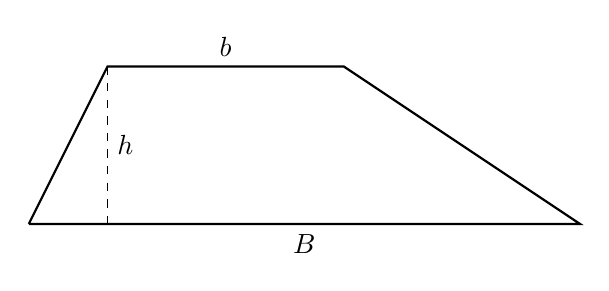
\begin{tikzpicture}
            \coordinate (A) at (0, 0);
            \coordinate (B) at (7, 0);
            \coordinate (C) at (4, 2);
            \coordinate (D) at (1, 2);
            \coordinate (O) at (1, 0);

            \draw[thick] (A) -- node[anchor=north] { $B$ } (B) -- (C) -- node[anchor=south] { $b$ } (D) -- (A);
            \draw[dashed] (D) -- node[anchor=west] { $h$ } (O);

        \end{tikzpicture}
    \end{figure}

\end{frame}

\begin{frame}[fragile]{Perímetro e área}

    \begin{itemize}
        \item A área de um trapézio é dada pela metade do produto entre a altura e a soma de
            suas bases, isto é,
        \[
            A = \frac{(B + b)h}{2}
        \]
        \pause

        \item Contudo, não há fórmulas para o perímetro que usam estas três medidas diretamente
        \pause

        \item Se as medidas dos lados não forem conhecidas, deve-se usar o Teorema de
            Pitágoras para deduzir as medidas ausentes
        \pause
    \end{itemize}

    \inputcode{cpp}{codes/trapezium.cpp}
\end{frame}
